\capitulo{4}{Técnicas y herramientas}

A continuación se mostrarán las técnicas y herramientas utilizadas para el desarrollo del proyecto. 
Tanto para la parte de documentación, como para la parte de desarrollo de la aplicación. 

\section{Técnicas}
\subsection{Scrum}
Scrum es una metodología para realizar el seguimiento de proyectos que comparte los principios del desarrollo ágil de partir de un concepto, seguir un desarrollo incremental (en \textit{sprints}) y cerrar el producto.

\subsubsection{Elementos}
\begin{itemize}
\item \textbf{Pila del producto o \textit{product backlog}:}
Es una lista de requisitos desde el punto de vista del cliente que comienza con una visión inicial del producto, pero que se irá incrementando a los largo del desarrollo.

\item \textbf{Pila del sprint o \textit{sprint backlog}:}
Conjunto de requisitos o tareas desde el punto de vista del desarrollador que el equipo de desarrollo del proyecto espera realizar durante el \textit{sprint}.

\item \textbf{Incremento:}
El incremento es el resultado del desarrollo de un \textit{sprint}, es una parte terminada y probada. 

\item \textbf{Gráfico de avance o \textit{burn-down chart}:}
Sirve para representar tanto el trabajo pendiente como el trabajo realizado durante un \textit{sprint} para ver la velocidad a la que se están completando las tareas. De este modo, se puede saber si se va dentro de la planificación o no.

\item \textbf{Gráfico de producto o \textit{burn-up chart}:}
Gráfico utilizado para ver el trabajo realizado respecto al total.

\item \textbf{Gráfico de velocidad o \textit{velocity chart}:}
Muestra la velocidad de trabajo durante el \textit{sprint}. Es útil para ir ajustando la previsión de tiempo en futuros \textit{sprints}.
\end{itemize}

\subsubsection{Roles}
Las personas que participan en el proyecto tienen asignado un rol. En el siguiente listado se pueden ver los distintos roles junto a una breve descripción de los mismos.
\begin{itemize}
\item \textbf{\textit{Scrum master}:}
Persona con conocimientos avanzados en la metodología Scrum que se encarga de que se cumpla correctamente el procedimiento. También es el encargado de dar formación y asesorar al resto de personal sobre Scrum.

\item \textbf{Propietario del producto o \textit{product owner}:}
Es la persona que hace de representación del cliente. Se encarga de la gestión de la pila del producto dando visión al producto con las historias de usuario y definiendo las prioridades de las mismas. Participa en cada reunión de planificación de los \textit{sprints}.

\item \textbf{Equipo de desarrollo:}
Es recomendable que no sea un equipo con un gran número de personal (entre 4 y 8 personas). El equipo debe trabajar de forma simultanea para cumplir las tareas indicadas en la reunión de planificación del \textit{sprint}.
\end{itemize}

En las figuras~\ref{ProcesoScrum1} y~\ref{ProcesoScrum2} se puede ver tanto un resumen del proceso seguido en Scrum como de los diferentes elementos que interactúan en el mismo.

\begin{figure}
	\centering
	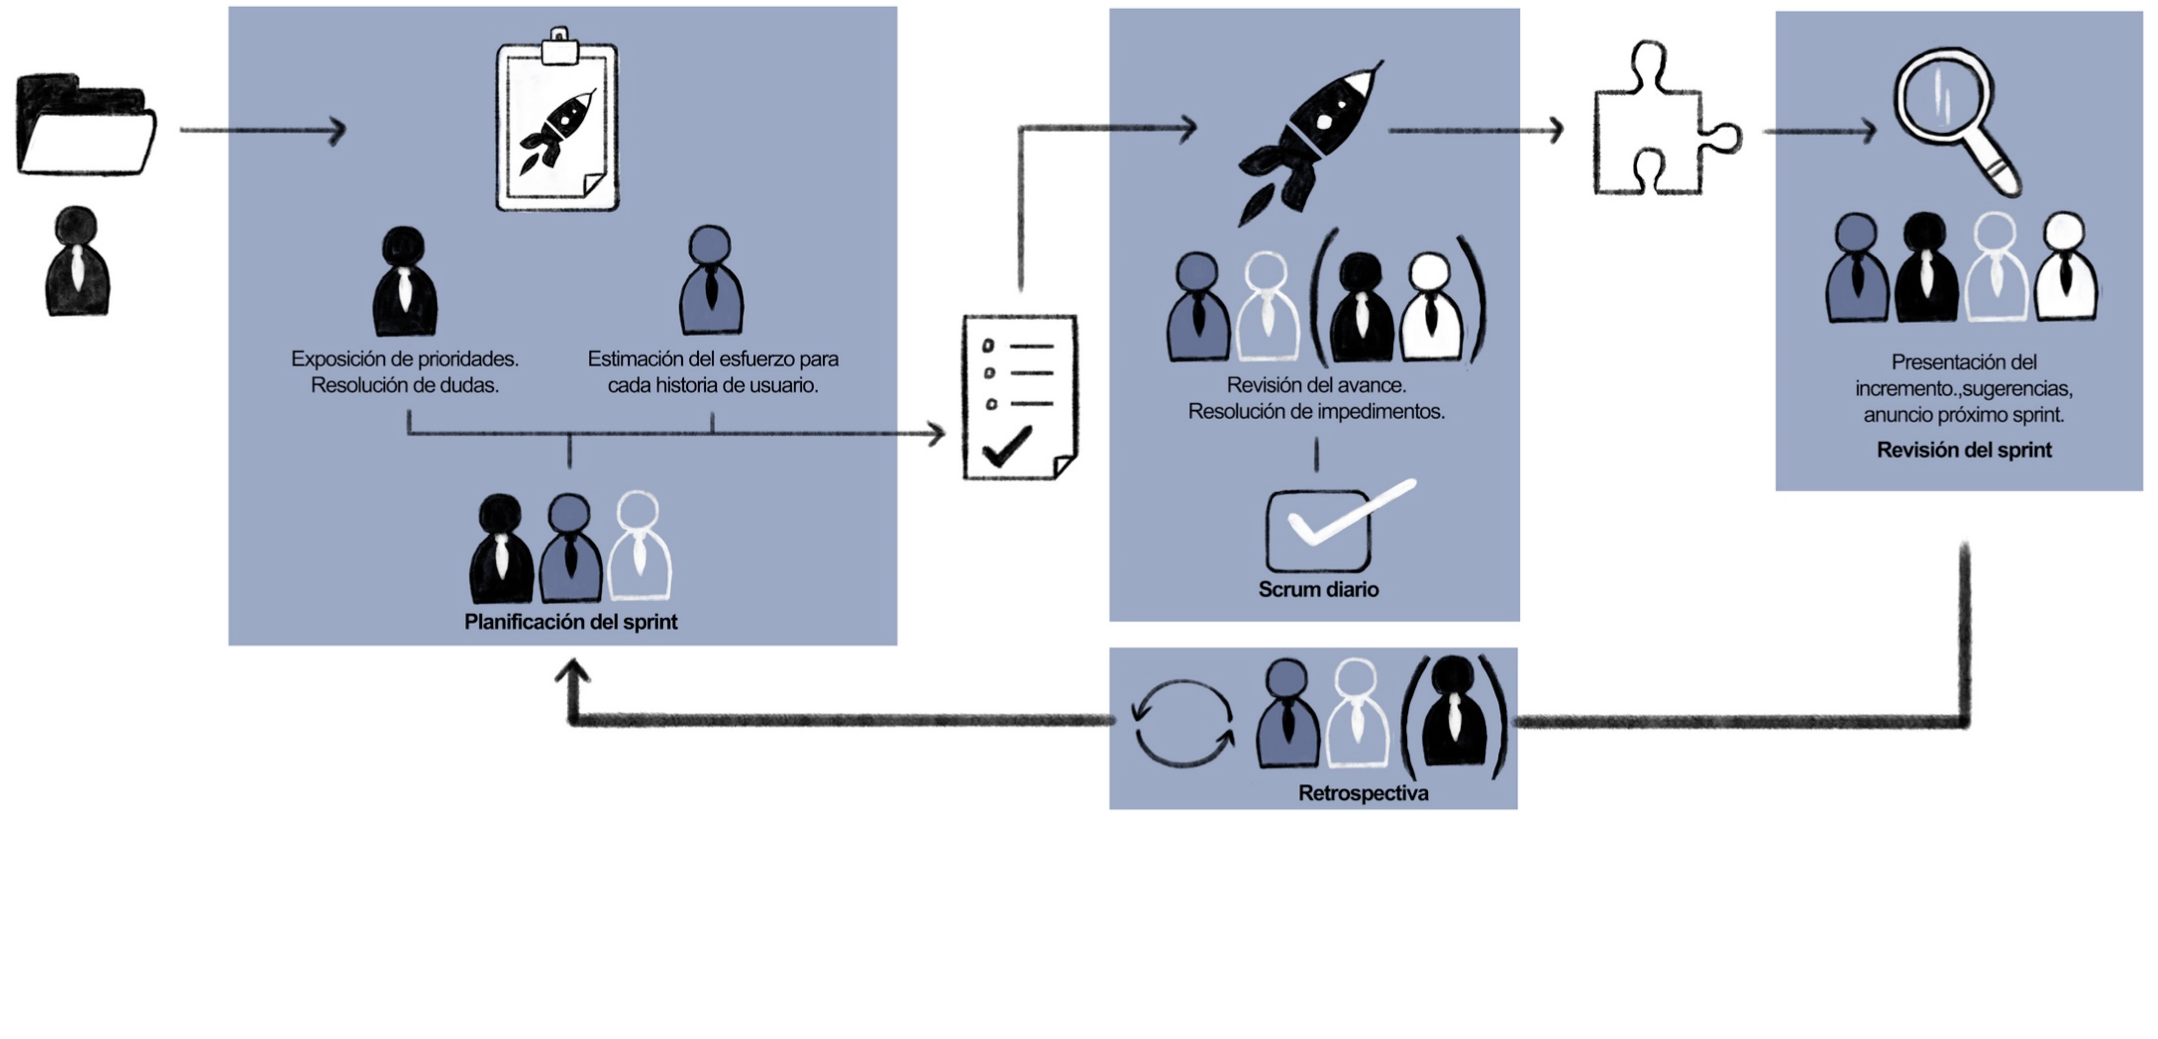
\includegraphics[width=\textwidth]{../img/Scrum/Scrum.png}
	\caption{\textit{Proceso seguido en Scrum \cite{scrum}}}\label{ProcesoScrum1}
\end{figure}


\begin{figure}
	\centering
	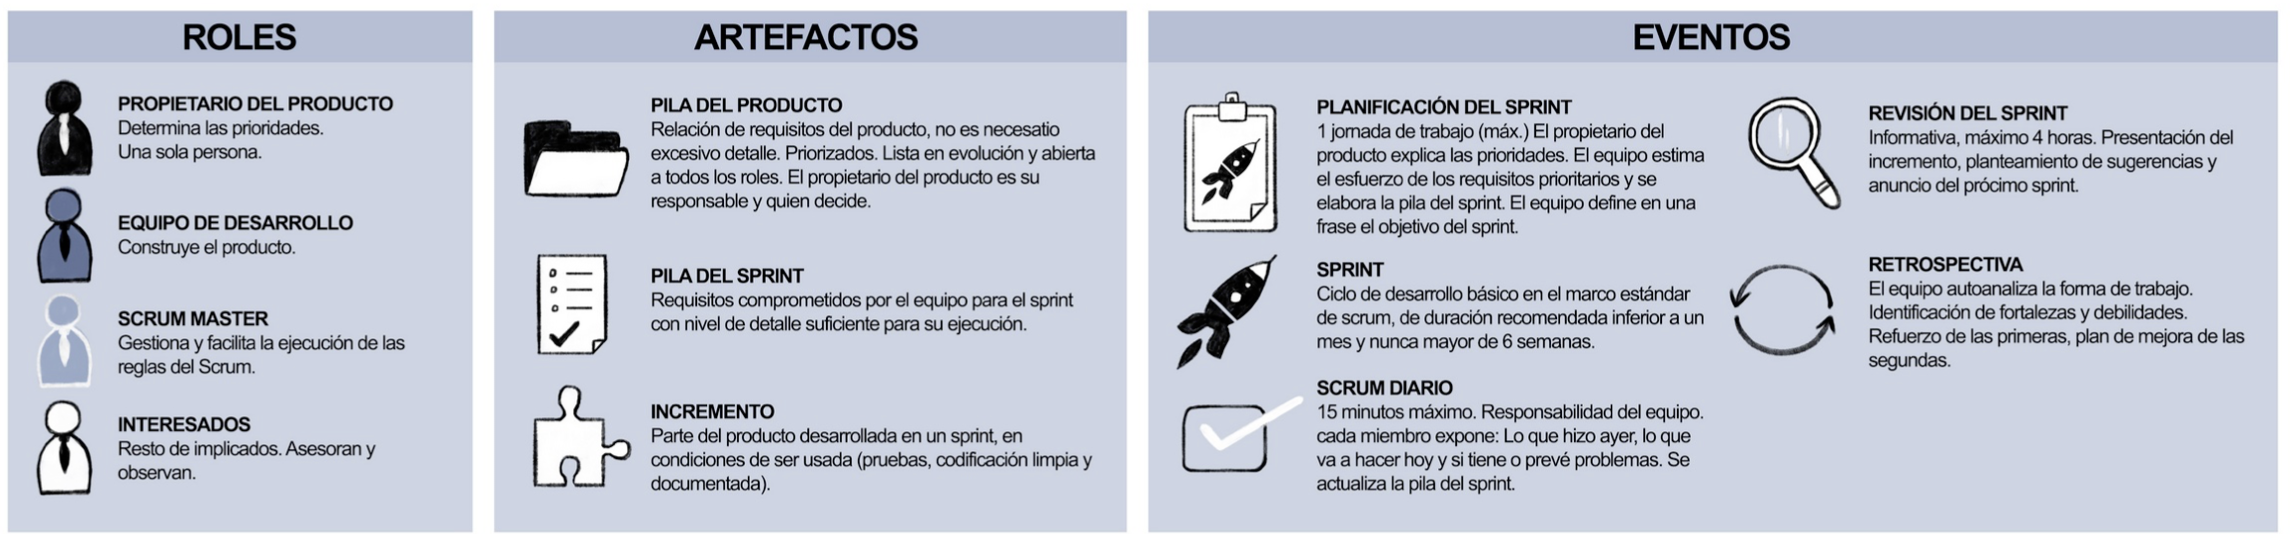
\includegraphics[width=\textwidth]{../img/Scrum/Scrum1.png}
	\caption{\textit{Explicación de los elementos del proceso \cite{scrum}}}\label{ProcesoScrum2}
\end{figure}


De forma resumida, para seguir la metodología Scrum es necesario que el propietario del producto genere inicialmente las historias de usuario, que se encontrarán en la pila del producto. Estas historias podrán aumentar a lo largo del desarrollo.

Con la pila del producto creada, todo el personal se reúne para planificar el \textit{sprint}. Estas reuniones son las que general la pila del \textit{sprint}.
Después de esta reunión, el equipo de desarrollo comienza a trabajar en las tareas que se ha comprometido para completarlas en el tiempo acordado. Cada día de trabajo se realiza una pequeña reunión de aproximadamente 15 minutos donde se expone el trabajo realizado, el trabajo que se va a hacer en el día, las dudas, etc., está reunión sirve para ir actualizando la pila del \textit{sprint}. 

Al final del \textit{sprint}, todo el personal se vuelve a reunir para presentar el incremento realizado y ver posibles cambios. Además, se fija el anuncio del próximo \textit{sprint} que comenzará de nuevo con una reunión de planificación.

Durante este proyecto se ha seguido una metodología Scrum con algunos cambios ya que no se hacían reuniones diarias ni los roles estaban tan marcados, pero la forma de trabajar era la misma con planificaciones y revisiones de \textit{sprints}.

\subsection{Web}
La web (\textit{World Wide Web}) es un sistema que permite la transmisión y acceso a datos y documentos a través de internet utilizando el protocolo HTTP para la comunicación y el lenguaje HTML para la representación de las páginas web~\cite{wiki:web}.

La tecnología web es una de las que más desarrollo ha sufrido en los últimos años. Esto ha provocado un cambio completo en nuestra forma de vida, afectando a aspectos como la búsqueda de información por Internet, realizar compras online, hacer trámites sin necesidad de acudir a una oficina, etc.,

 
\section{Herramientas}
\subsection{GitHub}
GitHub es una plataforma de alojamiento en la nube que permite llevar un control de versiones Git para los proyectos subidos. Además del control de versiones, GitHub posee distintas características como la creación de repositorios, el uso de \textit{issues}, \textit{Pull requests}, las páginas de \textit{wiki}, añadir distintos usuarios al repositorio con diferentes permisos, etc\cite{wiki:github}.

\subsection{ZenHub}
Extensión para navegador web que se integra con GitHub para permitir añadir los elementos de Scrum al repositorio. De esta manera se puede llevar un mejor seguimiento del trabajo realizado en el proyecto.

\subsection{Python}
Python es un popular lenguaje de programación que puede ser utilizado en diferentes ámbitos, entre ellos el desarrollo web. Algunas de las razones para utilizar este lenguaje es su facilidad de uso, la posibilidad de orientación a objetos y la amplia variedad de bibliotecas y frameworks, como puede ser Flask~\cite{python}.

Se estudió la posibilidad de uso de PHP para realizar la aplicación web, pero al final se decidió trabajar con Python debido a que es más conocido para los tutores del proyecto y a que, al utilizarlo durante el grado, es más fácil la adaptación para alumnos que en un futuro hagan nuevas versiones partiendo de este proyecto.

\subsection{Flask}
Como se ha comentado en el apartado anterior, Flask es un framework de Python que facilita la creación de aplicaciones web. Flask incluye el motor de plantillas Jinja2 que permite implementar código en las vistas de la aplicación de una forma cómoda y sencilla.

\subsection{JavaScript}
JavaScript es un lenguaje de programación interpretado débilmente tipado. Principalmente es conocido al ser utilizado en el lado del cliente para dar mejor interacción a páginas web estáticas, pero es mucho más potente de lo que se puede pensar y es utilizado en muchos más ámbitos. Incluso en la misma web, puede ser utilizado en el lado servidor mediante el entorno de ejecución Node.js. Esto permite que una aplicación web pueda estar completamente escrita en JavaScript~\cite{javascript}.

\subsection{HTML}
HTML es el <<Lenguaje de Marcas de Hipertexto>> utilizado por la \textit{World Wide Web} para representar las páginas web. Puede ser combinado con diferentes tecnologías como CSS para dar una apariencia diferente o JavaScript para poder interactuar de forma dinámica.

\subsection{CSS}
CSS, también conocido como <<Hojas de Estilo en Cascada>>, es un lenguaje de estilos utilizado para mejorar la apariencia de los ficheros HTML. Gracias a CSS se puede dar rienda suelta al diseño y hacer páginas web completamente diferentes.

\subsection{Bibliotecas / \textit{plugins}}
\begin{itemize}
\item\textbf{SQLAlchemy}

Biblioteca de SQL para Python que incluye una versión para el \textit{framework} Flask que permite su completa integración. 
SQLAlchemy contiene un conjunto de herramientas SQL que permiten el mapeo objeto-relacional, \textit{Object Relational Mapper (ORM)}. 
Esto permite que con un conjunto de expresiones requeridas por la biblioteca, se creen clases de objetos en Python que serán transformadas a tablas de una forma prácticamente abstracta para el desarrollador. 
Además, al estar los objetos vinculados a registros de una tabla SQL, cuenta con métodos para realizar distintas operaciones SQL como búsquedas, inserciones, eliminaciones, etc., sin tener que escribir sentencias SQL~\cite{sqlAlchemy}.

\item\textbf{Grid.js}

Grid.js es un \textit{plugin} de JavaScript que ayuda con el tratamiento de tablas. 
Gracias a esta biblioteca se pueden crear tablas con búsqueda, ordenamiento, redimensión de columnas, etc., de una forma sencilla gracias a sus herramientas. 
Además, Grid.js se puede incluir con \textit{frameworks} como Reac, Angular o Vue, pero también puede ser utilizado con JavaScript \textit{vanilla}.


Antes de la elección de este \textit{plugin} se estuvo valorando el uso de otro llamado DataTables. Al final se decidió utilizar Grid.js a pesar de que DataTables es más completo.

Algunas de las razones son la siguientes:
\begin{itemize}
\item Para utilizar Grid.js no es necesaria la biblioteca jQuery mientras que para DataTables sí. La dependencia de otras bibliotecas puede dar problemas en un futuro, además de que el rendimiento de JavaScript \textit{vanilla} es algo superior.
\item Aunque esto se pueda cambiar, la estética de Grid.js me parece más moderna.
\item Para este proyecto no eran necesarias muchas de las funcionalidades que aporta DataTables.
\item En su repositorio en GitHub, se puede ver por los \textit{commits} realizados que es un proyecto en continuo desarrollo.
\end{itemize}
\end{itemize}

\subsection{Software}
\begin{itemize}
\item\textbf{Pincel Project}

Es un programa de ordenador gratuito y de código abierto que permite la creación de los prototipos de las vistas de una aplicación de una forma cómoda, arrastrando distintos elementos a la pantalla y modificándolos para que queden al gusto del creador. 
Cuenta con versiones para Windoes, Linux y macOS.
Por defecto, el software cuenta con objetos suficientes para crear los prototipos de las vistas de una aplicación. 
Sin embargo, es posible cargar más de estos objetos creados por la comunidad o por uno mismo, como pueden ser nuevos botones, campos de entrada, menús, etc.

\item\textbf{Draw.io}

Aplicación web que permite la creación de diagramas utilizando diferentes figuras geométricas. 
Además cuenta con objetos ya creados para crear diagramas utilizando UML, diagramas entidad-relación, diagramas relacionales, etc. 
Esta aplicación permite una personalización avanzada por lo que es muy útil para crear cualquier tipo de diagrama. 
Además, al ser una aplicación web no requiere de ningún tipo de instalación aunque si que cuenta con una versión de escritorio para Windows, Linux, macOS y Chrome OS.

\item\textbf{PyCharm}

Es un entorno de desarrollo integrado (IDE) que pertenece a la empresa JetBrains y que está creado para trabajar el proyectos basados en el lenguaje de programación Python. 
Cuenta con una licencia de uso gratuita con funciones limitadas, aunque para estudiantes regalan un año de licencia completa para todos los productos de la empresa.

PyCharm es uno de los IDE más completos y avanzados para el desarrollo con Python, ya que cuenta con una gran cantidad de características que facilitan el trabajo y ayudan a ahorrar tiempo. 
Además, a la hora de crear proyectos se puede indicar el tipo de \textit{framework} a utilizar, lo que hará que cargue de forma automática todos los paquetes necesarios y creará una versión simple del proyecto desde la que empezar a trabajar. 
Esto ahorra mucho tiempo al no tener que ir buscando e instalando los paquetes necesarios desde distintos repositorios. 
\end{itemize}
\subsection{}
